% Add to the preamble:  \newcommand{\MSc}{MeshSplatting-cap\xspace}
\section{Experiments}
\label{sec:exp}

\noindent\textbf{Datasets and protocol.} We use Mip-NeRF~360~\cite{barron2022mipnerf360} (9 scenes), Tanks and Temples~\cite{knapitsch2017tanks} (truck, train), Deep Blending~\cite{hedman2018deep} (drjohnson, playroom) and NeRF-Synthetic~\cite{mildenhall2020nerf} (8 objects), 21 scenes in total. The training settings of \MS are unchanged: 30k iterations, images downsampled by 2 for indoor scenes and by 4 for outdoor scenes, the standard test split, and a black background for NeRF-Synthetic. Quality is measured by the PSNR, SSIM and LPIPS of the test views rendered from the decoded mesh file. The FP32 model is the mesh that \MS produces with its released settings, stored in 32-bit floats (our reproduction).

\noindent\textbf{Settings.} \BM uses one setting for all 21 scenes and all target sizes. The size probe runs every 500 iterations from 12.5k to 29.5k, and the growth in Phase~1 aims at $\alpha = 1.35$ times the target. BM-Codec uses SH codebooks of $K = 4{,}096$ and $K_r = 256$ codewords and 7 bits for the DC color. Over the range of file sizes that we test, this choice is at most 0.07\dB below the best combination of codebook sizes, and 8 bits for the DC color would make the files 4\% larger for 0.03\dB (supplement). Positions use 14 to 18 bits depending on the scene (14 for NeRF-Synthetic, 14--16 for Mip-NeRF~360, 15 for Deep Blending, 18 for Tanks and Temples). All baselines use the same position precision as \BM on the same scene.

\noindent\textbf{Baselines.} No codec exists for meshes with SH colors, so we build the baselines from what is available. \MS has no size control. Its cap on the number of vertices is the only parameter that affects the size, so we lower the cap to obtain smaller meshes. We call this baseline \MSc. We also reduce the FP32 model by edge collapse after training. On these meshes we compare BM-Codec, the codec of \BM, with three baseline codecs: MPEG TFAN~\cite{mamou2009tfan}, Draco~\cite{draco} and a quantized PLY compressed with zstd. Each baseline codec is run with the SH coefficients quantized to 8, 6 and 4 bits, and its rate--quality curve is the convex hull of its points. We report the quality gain at the same size by BD-PSNR and the size reduction at the same quality by BD-rate, computed with piecewise-linear interpolation over the logarithm of the file size.

%------------------------------------------------------------------
\begin{figure*}[t]\centering
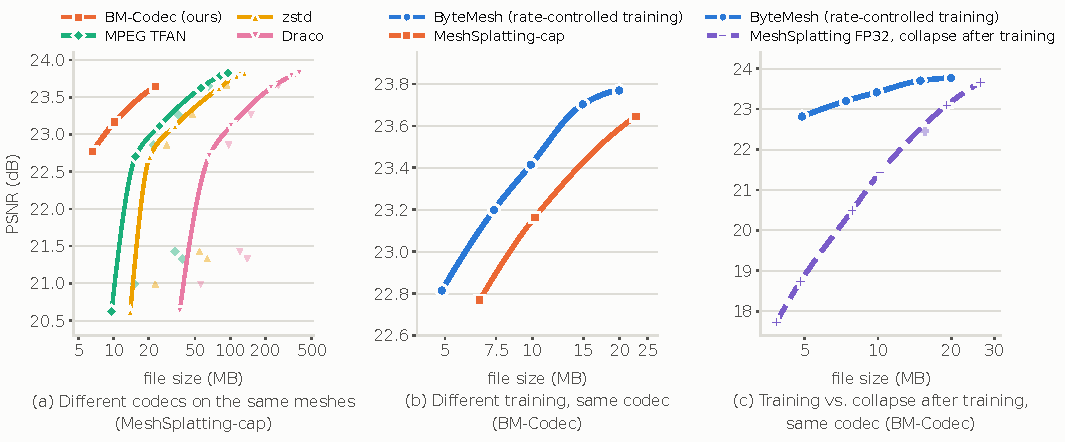
\includegraphics[width=\linewidth]{figures/fig_rd_three_v3.pdf}
\caption{\textbf{Rate--distortion on Mip-NeRF~360 and Tanks and Temples} (mean over 11 scenes). One factor changes in each panel: (a)~the codec, (b)~the training, (c)~when the mesh is reduced. The panels have different PSNR ranges.}
\label{fig:rd}
\end{figure*}

\begin{table}[t]\centering\footnotesize
\caption{\textbf{Bjontegaard deltas}, computed per scene and averaged. Top: BM-Codec against each baseline codec on the same meshes. Bottom: \BM against \MSc, both with BM-Codec. Negative BD-rate: fewer bytes for the same PSNR. ``--'': no file size in common.}
\label{tab:bd}
\setlength{\tabcolsep}{3.5pt}
\begin{tabular}{@{}llcc@{}}
\toprule
meshes (scenes) & against & BD-PSNR & BD-rate \\
\midrule
\multicolumn{4}{@{}l}{BM-Codec against baseline codecs} \\
\multirow{3}{*}{\shortstack[l]{\MSc,\\Mip-NeRF 360, T\&T (11)}} & TFAN & $+1.37$ dB & $-63.4\%$ \\
 & zstd & $+1.68$ dB & $-73.3\%$ \\
 & Draco & -- & $-91.3\%$ \\
\multirow{3}{*}{\shortstack[l]{\MSc,\\Deep Blending (2)}} & TFAN & $+1.67$ dB & $-62.5\%$ \\
 & zstd & $+1.84$ dB & $-73.1\%$ \\
 & Draco & -- & $-92.5\%$ \\
\multirow{3}{*}{\shortstack[l]{\MSc,\\NeRF-Synthetic (8)}} & TFAN & $+0.68$ dB & $-32.5\%$ \\
 & zstd & $+1.18$ dB & $-46.5\%$ \\
 & Draco & -- & $-87.2\%$ \\
\multirow{3}{*}{\shortstack[l]{collapse after training,\\Mip-NeRF 360, T\&T (11)}} & TFAN & $+2.66$ dB & $-60.5\%$ \\
 & zstd & $+3.77$ dB & $-72.7\%$ \\
 & Draco & $+5.34$ dB & $-88.1\%$ \\
\midrule
\multicolumn{4}{@{}l}{\BM against \MSc + BM-Codec} \\
Mip-NeRF 360, T\&T (11) & & $+0.30$ dB & $-31.3\%$ \\
Deep Blending (2) & & $+0.23$ dB & $-22.8\%$ \\
NeRF-Synthetic (8) & & $+0.29$ dB & $-21.1\%$ \\
all (21) & & $+0.29$ dB & $-26.9\%$ \\
\bottomrule
\end{tabular}
\end{table}
%------------------------------------------------------------------

\subsection{Compressing meshes generated by MeshSplatting with variable vertex caps}
\label{sec:codec}
We first evaluate the compression efficiency of BM-Codec. All codecs are applied to the same meshes, so that only the codec differs (Fig.~\ref{fig:rd}a). The meshes come from \MSc with caps of 0.6, 1.08 and 3 million vertices and from the default setting of \MS; before coding, stored in 32-bit floats, they take 130, 216, 519 and 609~MB and reach 22.91, 23.36, 23.92 and 23.96\dB. Table~\ref{tab:bd} (top) gives the Bjontegaard deltas of BM-Codec against each baseline codec. On Mip-NeRF~360 and Tanks and Temples, BM-Codec needs 63\% fewer bytes than TFAN, 73\% fewer than zstd and 91\% fewer than Draco at the same PSNR. The results on Deep Blending are similar. On NeRF-Synthetic the reductions are 33\%, 47\% and 87\%. On the meshes obtained by collapse after training (92, 199 and 392~MB and 18.62, 21.30 and 23.23\dB before coding), the reductions are 61\%, 73\% and 88\%. The rate--distortion curves on Deep Blending and NeRF-Synthetic are in the supplement.

The lossy steps of BM-Codec (vector quantization of the SH coefficients and quantization of positions and color) lower the PSNR by 0.15, 0.20 and 0.27\dB on average on the three \MSc meshes, relative to the same meshes before coding.

\subsection{Gain of rate-controlled training}
\label{sec:rd}
We now fix the codec to BM-Codec and compare the training (Fig.~\ref{fig:rd}b). \BM is better than \MSc on 20 of the 21 scenes and equal on one (treehill). The BD-PSNR is $+0.29$\dB on average and the BD-rate is $-26.9\%$ (Table~\ref{tab:bd}, bottom).

\begin{table}[t]\centering\footnotesize
\caption{\textbf{\BM at three target sizes and the FP32 model of \MS}, dataset means over single runs; size in MB. Size error is $|\text{file}-\text{target}|/\text{target}$. All targets are in the supplement. $^\dagger$Two objects (ficus, mic) are fully represented by about 2 to 2.6~MB and do not grow further.}
\label{tab:main}
\setlength{\tabcolsep}{3.2pt}
\begin{tabular}{@{}llccccc@{}}
\toprule
dataset & target & size & err. & PSNR & SSIM & LPIPS \\
\midrule
\multirow{4}{*}{\shortstack[l]{Mip-NeRF\\360 (9)}} & 20 & 19.91 & 0.8\% & 24.46 & 0.707 & 0.406 \\
 & 10 & 9.87 & 1.5\% & 24.06 & 0.678 & 0.453 \\
 & 5 & 4.85 & 2.9\% & 23.42 & 0.635 & 0.506 \\
 & FP32 & 642 & -- & 24.81 & 0.731 & 0.309 \\
\midrule
\multirow{4}{*}{\shortstack[l]{Tanks and\\Temples (2)}} & 20 & 20.01 & 0.2\% & 20.64 & 0.750 & 0.332 \\
 & 10 & 9.94 & 0.6\% & 20.51 & 0.736 & 0.361 \\
 & 5 & 4.96 & 0.8\% & 20.09 & 0.703 & 0.408 \\
 & FP32 & 459 & -- & 20.64 & 0.760 & 0.272 \\
\midrule
\multirow{4}{*}{\shortstack[l]{Deep\\Blending (2)}} & 20 & 19.93 & 0.9\% & 27.01 & 0.840 & 0.450 \\
 & 10 & 9.93 & 0.7\% & 26.69 & 0.833 & 0.474 \\
 & 5 & 4.99 & 0.3\% & 26.04 & 0.821 & 0.498 \\
 & FP32 & 772 & -- & 27.23 & 0.842 & 0.337 \\
\midrule
\multirow{4}{*}{\shortstack[l]{NeRF-\\Synthetic (8)}} & 4$^\dagger$ & 3.56 & 11.3\% & 31.20 & 0.952 & 0.069 \\
 & 2.5$^\dagger$ & 2.43 & 3.2\% & 31.10 & 0.951 & 0.069 \\
 & 1.5 & 1.50 & 0.3\% & 30.45 & 0.945 & 0.079 \\
 & FP32 & 65.7 & -- & 31.17 & 0.955 & 0.063 \\
\bottomrule
\end{tabular}
\end{table}

\noindent\textbf{No prior knowledge of the scene.} With \MSc, the same cap gives files that differ by a factor of 1.3 to 2.0 across the captured scenes (5.8--7.5~MB at 0.6 million vertices, 20.0--39.8~MB at the default 4 million; supplement). The cap for a wanted file size therefore depends on the scene. \BM takes the file size as its input and uses the same controller settings everywhere. Table~\ref{tab:main} lists its results. On the captured scenes, all 65 runs end within 10\% of the target, and the mean error is at most 2.9\% for every dataset and target. On the objects, 21 of 24 runs end within 10\%. The three others are ficus and mic at 2.5 or 4~MB: these objects are fully represented by about 2 to 2.6~MB, so the file stays below the target.

\noindent\textbf{Against the FP32 model.} At the highest target of 20~MB, the files of \BM are 31 times smaller than the FP32 model on Mip-NeRF~360 and Tanks and Temples (609~MB on average), for a PSNR loss of 0.28\dB. On NeRF-Synthetic, the 3.6~MB files match the PSNR of the 65.7~MB FP32 models.

\subsection{Collapse after training}
\label{sec:simp}
Fig.~\ref{fig:rd}c compares \BM with the FP32 model reduced by edge collapse after training, both written by BM-Codec. At the same vertex count, \MSc is already better than collapse after training on 127 of 128 scene--budget pairs, by 1.86\dB on average. The loss grows as the mesh is reduced: 0.5\dB for files of 12 to 23~MB, 1.9\dB at 8 to 12~MB and 3.9\dB below 8~MB. The reason is that each pixel is covered by one opaque triangle. After a collapse, the neighboring triangles have not been trained for their new shape, and no other primitive covers the error. Fig.~\ref{fig:qual} shows the three ways to reach the same file size on three scenes.

\subsection{Other representations}
\label{sec:cross}

\begin{table}[t]\centering\footnotesize
\caption{\textbf{Other representations on Mip-NeRF~360}; size in MB. Gaussian rows are published numbers collected in~\cite{hacpp2025} and are given for reference. Mesh rows are published numbers collected in~\cite{meshsplatting2025}. \MS FP32 is our reproduction.}
\label{tab:cross}
\setlength{\tabcolsep}{4pt}
\begin{tabular}{@{}lcccc@{}}
\toprule
method & PSNR & SSIM & LPIPS & MB \\
\midrule
3DGS~\cite{kerbl2023gaussians} & 27.46 & 0.812 & 0.222 & 750.9 \\
Compact3DGS~\cite{compact3dgs2024} & 27.08 & 0.798 & 0.247 & 48.80 \\
HAC++~\cite{hacpp2025}, low & 27.60 & 0.803 & 0.253 & 8.34 \\
HAC++, high & 27.82 & 0.811 & 0.231 & 18.48 \\
\midrule
GOF mesh~\cite{gof2024} & 20.78 & 0.573 & 0.465 & 1500 \\
RaDe-GS mesh~\cite{rade2024} & 23.56 & 0.668 & 0.361 & 1100 \\
MiLo~\cite{milo2025} & 24.09 & 0.688 & 0.323 & 253 \\
\MS FP32~\cite{meshsplatting2025} & 24.81 & 0.731 & 0.309 & 642 \\
\midrule
\BM, 20 MB & 24.46 & 0.707 & 0.406 & 19.9 \\
\BM, 10 MB & 24.06 & 0.678 & 0.453 & 9.9 \\
\BM, 5 MB & 23.42 & 0.635 & 0.506 & 4.9 \\
\bottomrule
\end{tabular}
\end{table}

Table~\ref{tab:cross} compares \BM with other representations on Mip-NeRF~360. Among the methods that output a mesh, \BM is the only one below 20~MB. At 20~MB it is 0.35\dB below the FP32 model of \MS, and it is above MiLo, RaDe-GS and GOF with files 13 to 75 times smaller. Compressed Gaussians remain better at the same size: HAC++ is 3.4 to 4.2\dB higher in PSNR. This gap comes from the representation (opaque triangles against semi-transparent Gaussians) and is already present before compression, between \MS and 3DGS. What the mesh offers in exchange is a standard indexed triangle mesh that any engine renders without sorting. In a WebGL viewer on a laptop (Apple M2 Max, $1920 \times 958$), the 5, 10 and 20~MB files of garden, room and bicycle render in 1.1, 1.3 and 2.0~ms per frame on average.

\subsection{Complexity}
\label{sec:time}

\begin{table}[t]\centering\footnotesize
\caption{\textbf{Encoding and decoding time} in seconds, mean over 11 scenes (about 0.93 million vertices each). Fitting the codebooks runs on a GPU; everything else on a CPU. TFAN is called once for both directions.}
\label{tab:time}
\begin{tabular}{@{}lcc@{}}
\toprule
codec & encode & decode \\
\midrule
zstd (quantized PLY) & 15.4 & 0.2 \\
Draco & 16.6 & 3.8 \\
TFAN & \multicolumn{2}{c}{8.2 (both)} \\
BM-Codec, codebook fitting & 90 & -- \\
BM-Codec, entropy coding & 4.6 & 3.7 \\
\bottomrule
\end{tabular}
\end{table}

Table~\ref{tab:time} gives the encoding and decoding times. The codebooks of BM-Codec are fitted per scene, which takes about 90 seconds and includes the search for the nearest codeword of every vertex. With this step, encoding takes about 95 seconds in total and is slower than the baseline codecs. Decoding takes 3.7 seconds, similar to Draco. One training run of \BM takes 48.8 minutes on average on the 13 captured scenes (one L40S GPU), including the size probes.

\subsection{Ablation}
\label{sec:abl}

\begin{table}[t]\centering\footnotesize
\caption{\textbf{Selection rules}: PSNR change (dB) when the split rule or the collapse rule is replaced by the importance score of \MS. Target 10~MB, one run each; every file is within 3\% of the target.}
\label{tab:abl}
\setlength{\tabcolsep}{3.2pt}
\begin{tabular}{@{}lcccccc@{}}
\toprule
 & garden & room & bicycle & kitchen & truck & mean \\
\midrule
split by importance & $-0.17$ & $-0.43$ & $-0.29$ & $-0.62$ & $-0.20$ & $-0.34$ \\
collapse by importance & $-0.78$ & $-2.38$ & $-0.08$ & $-5.68$ & $-0.69$ & $-1.92$ \\
\bottomrule
\end{tabular}
\end{table}

\noindent\textbf{Selection rules.} \BM uses the per-triangle error $e_t$ in both rules: it splits the triangles with the largest error, and collapses the edges with the least error per byte saved. Table~\ref{tab:abl} replaces $e_t$ in one rule at a time by the importance score that \MS computes for each triangle, and keeps everything else. Both replacements lower the PSNR on all five scenes, by 0.34\dB on average for the split rule and 1.92\dB for the collapse rule.

\noindent\textbf{Collapse schedule.} \BM probes the file size every 500 iterations until 29.5k and removes the measured excess each time. In a variant, the collapse rounds stop at 19.5k, and each round also removes the growth of the file that it predicts for the rest of training. We ran both versions on the 11 scenes of Mip-NeRF~360 and Tanks and Temples at three targets (33 runs each). With \BM the mean size error is 1.5\% instead of 4.3\%, and 23 runs instead of 7 end within 2\% of the target. At the same file size, the PSNR of \BM is higher by 0.02, 0.06 and 0.13\dB at 20, 10 and 5~MB.

\begin{table}[t]\centering\footnotesize
\caption{\textbf{Effect of the growth aim $\alpha$}. Target 10~MB, one run each.}
\label{tab:alpha}
\setlength{\tabcolsep}{5pt}
\begin{tabular}{@{}lcccc@{}}
\toprule
 & \multicolumn{2}{c}{garden} & \multicolumn{2}{c}{room} \\
\cmidrule(lr){2-3}\cmidrule(lr){4-5}
$\alpha$ & size (MB) & PSNR (dB) & size (MB) & PSNR (dB) \\
\midrule
1.0 & 8.46 & 23.33 & 8.72 & 27.65 \\
1.2 & 9.94 & 23.57 & 10.03 & 27.90 \\
1.35 & 10.00 & 23.67 & 9.99 & 27.99 \\
1.5 & 9.96 & 23.76 & 9.70 & 27.84 \\
\bottomrule
\end{tabular}
\end{table}

\noindent\textbf{Growth aim.} \BM grows the mesh to $\alpha = 1.35$ times the target and then removes the excess. Table~\ref{tab:alpha} varies $\alpha$. With $\alpha = 1.0$, the file ends 13\% to 15\% below the target and no collapse round is active: vertices are lost between the end of densification and the triangulation, and nothing can add them back. Growing past the target is therefore necessary. Between 1.2 and 1.5, the file is on target and the PSNR changes by less than 0.2\dB. We use $\alpha = 1.35$ for all scenes.

\begin{table}[t]\centering\footnotesize
\caption{\textbf{Codec design choices}, mean over 11 scenes (meshes of about one million vertices). The first row of each block is the codec used for all other results.}
\label{tab:codec-abl}
\setlength{\tabcolsep}{4pt}
\begin{tabular}{@{}llcc@{}}
\toprule
attribute & coding method & bits/vertex & size change \\
\midrule
\multirow{4}{*}{positions} & one earlier neighbor & 22.6 & -- \\
 & previous vertex & 23.2 & $+0.7\%$ \\
 & parallelogram & 23.5 & $+1.0\%$ \\
 & mean of earlier neighbors & 21.6 & $-1.1\%$ \\
\midrule
\multirow{2}{*}{DC color} & zstd, no prediction & 12.6 & -- \\
 & mean of earlier neighbors & 11.3 & $-1.5\%$ \\
\midrule
\multirow{3}{*}{SH indices} & neighbor candidates & 17.6 & -- \\
 & no neighbor information & 17.4 & $-0.3\%$ \\
 & fixed length & 20.0 & $+2.8\%$ \\
\bottomrule
\end{tabular}
\end{table}

\noindent\textbf{Codec design choices.} Table~\ref{tab:codec-abl} measures alternatives for the lossless coding of three vertex attributes on the same meshes. For positions, BM-Codec predicts a vertex from one earlier neighbor: among the connected vertices that are already decoded, the one with the smallest index. The decoder finds it from the connectivity, so no bits are spent on the choice. This is better than the previous vertex and than parallelogram prediction on all 11 scenes. Predicting from the mean of all earlier neighbors is better still, and the same holds for the DC color. For the SH indices, using the indices of the neighbors as candidates does not help. Coding each index directly with an arithmetic coder, whose symbol probabilities are updated as the indices are coded, gives slightly smaller streams. Together, the better variants would make the files about 2.9\% smaller. They are not used in the reported results, so the reported sizes are conservative.

\subsection{Limitations}
\label{sec:limits}
LPIPS degrades more than PSNR: on Mip-NeRF~360 it rises from 0.309 for the FP32 model to 0.406 at 20~MB and 0.506 at 5~MB. Training does not include the quantization of the colors. The per-triangle error is accumulated at every training iteration on the unquantized mesh, and the codebooks are fitted only inside the size probes, on a copy that is discarded, and once after training. Encoding is slower than the baseline codecs because the codebooks are fitted per scene. The position precision is set by hand for each scene. A scene that is fully represented below the target stays below it. NeRF-Synthetic is evaluated on a black background, so its numbers cannot be compared with published results on a white background. The ablation of the growth aim uses two scenes and one run each.

%==================================================================
% SUPPLEMENT (paste into the appendix file)
%==================================================================
% \begin{figure*}[t]\centering
% 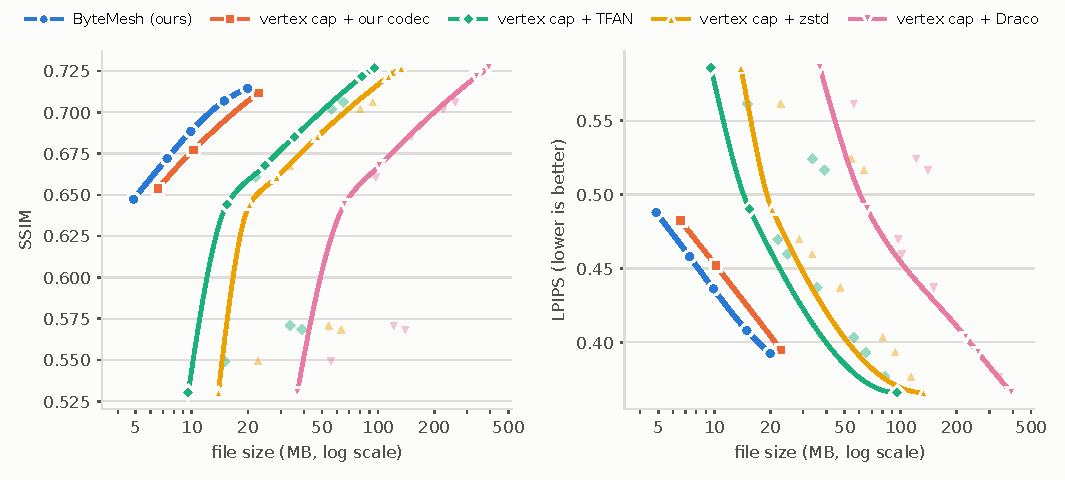
\includegraphics[width=\linewidth]{figures/fig_rd_ssim_lpips_v2.pdf}
% \caption{\textbf{SSIM and LPIPS against file size} on Mip-NeRF~360 and Tanks and Temples (mean over 11 scenes), for the baselines trained with a vertex cap. Same runs as Fig.~\ref{fig:rd}a.}
% \label{fig:rd-ssim-lpips}
% \end{figure*}
%
% \begin{figure*}[t]\centering
% 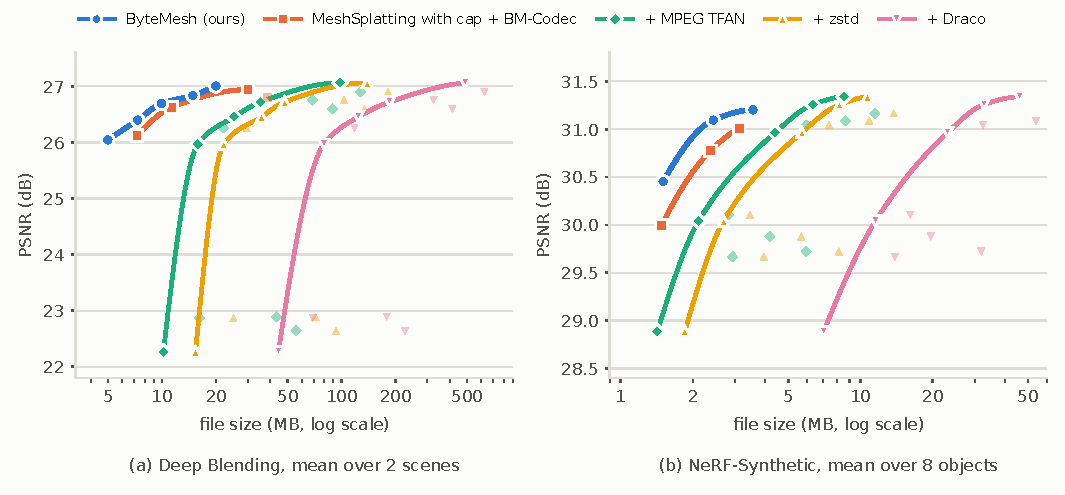
\includegraphics[width=\linewidth]{figures/fig_rd_db_obj_v1.pdf}
% \caption{\textbf{Rate--distortion on NeRF-Synthetic} (mean over 8 objects), baselines trained with a vertex cap.}
% \label{fig:rd-objects}
% \end{figure*}
%
% \noindent\textbf{Codebook size.} Table~\ref{tab:kr} compares five sizes of the two codebooks on the 11 scenes of Mip-NeRF~360 and Tanks and Temples at four file sizes. Removing the residual codebook saves about 8\% of the bytes and loses 0.12 to 0.15\dB. Enlarging the codebooks to 16{,}384 and 1{,}024 makes the files 12\% to 49\% larger for a gain of 0.06 to 0.07\dB. If the best size were chosen for each scene and each file size, the gain over the fixed choice would be between 0.02 and 0.15\dB per scene (0.08\dB on average); the largest gains are at the smallest files, where 1{,}024 + 256 is more efficient. The sweep was run on meshes from an earlier version of our training; the codec is the same.
%
% \begin{table*}[t]\centering\footnotesize
% \caption{\textbf{Codebook size.} Change in file size and PSNR (dB) against $K{=}4{,}096$, $K_r{=}256$, mean over 11 scenes, at four file sizes (size of the default file in the header).}
% \label{tab:kr}
% \begin{tabular}{@{}lcccc@{}}
% \toprule
% $K + K_r$ & 4.5 MB & 9.4 MB & 20.4 MB & 27.0 MB \\
% \midrule
% 4{,}096 + 0 & $-8.0\%$, $-0.12$ & $-8.4\%$, $-0.14$ & $-8.7\%$, $-0.15$ & $-8.9\%$, $-0.15$ \\
% 1{,}024 + 256 & $-12.8\%$, $-0.05$ & $-7.6\%$, $-0.05$ & $-5.0\%$, $-0.07$ & $-4.4\%$, $-0.07$ \\
% 4{,}096 + 256 & \multicolumn{4}{c}{reference} \\
% 4{,}096 + 1{,}024 & $+4.4\%$, $+0.02$ & $+3.3\%$, $+0.02$ & $+2.7\%$, $+0.03$ & $+2.7\%$, $+0.03$ \\
% 16{,}384 + 1{,}024 & $+49\%$, $+0.06$ & $+27\%$, $+0.06$ & $+15\%$, $+0.07$ & $+12\%$, $+0.07$ \\
% \bottomrule
% \end{tabular}
% \end{table*}
%
% \noindent\textbf{Prediction of the DC color.} In the codec used for all results, the DC color is quantized to 7 bits and compressed with zstd. We also coded it with a prediction from the vertices decoded earlier (the rounded mean of the earlier neighbors) and a context-adaptive binary arithmetic coder, and verified an exact round trip. On the 11 scenes of Mip-NeRF~360 and Tanks and Temples, the DC stream goes from 12.6 to 11.3 bits per vertex ($-10.4\%$) and the file becomes 1.46\% smaller on average ($0.84\%$ to $2.00\%$). The reported file sizes do not include this gain.
%
% \begin{figure}[t]\centering
% 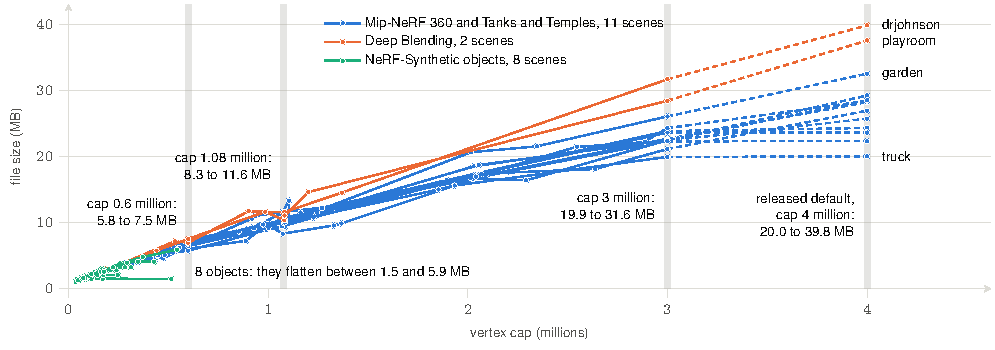
\includegraphics[width=\linewidth]{figures/fig_cap_instability.pdf}
% \caption{\textbf{File size against the vertex cap}, one line per scene, BM-Codec. Dashed segments lead to the released default of 4 million. The numbers on top give the range of file sizes over the captured scenes at four caps.}
% \label{fig:cap}
% \end{figure}
%
% \begin{figure}[t]\centering
% 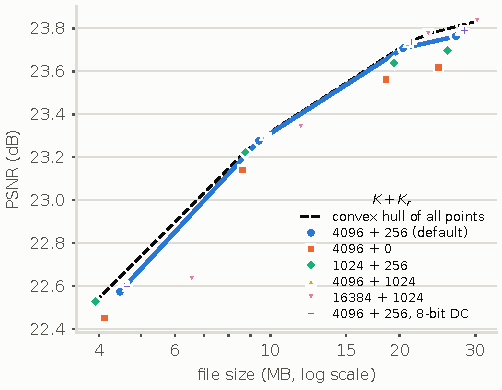
\includegraphics[width=\linewidth]{figures/fig_codebook_sweep_v1.pdf}
% \caption{\textbf{Codebook size.} Each point is the mean over 11 scenes of one combination of mesh size (four sizes) and codec setting (six settings). Dashed: convex hull of all 24 points. Blue: the setting used in this paper, which is at most 0.07\dB below the hull. The meshes come from an earlier version of our training; the codec is the same.}
% \label{fig:kr}
% \end{figure}
%
% Also for the supplement: the full table of \BM at all five targets (Table tab:main of the v2 file), Tanks and Temples and NeRF-Synthetic columns of the comparison with other representations, and the 4-row qualitative figure.
